
%(BEGIN_QUESTION)
% Copyright 2009, Tony R. Kuphaldt, released under the Creative Commons Attribution License (v 1.0)
% This means you may do almost anything with this work of mine, so long as you give me proper credit

A flow transmitter measuring process liquid flow through this valve array registers 5 GPM (out of a 0-1800 GPM measurement range) when the control valve is fully closed.  An operator shows you this, declaring the control valve to be leaking (internally).

$$\includegraphics[width=15.5cm]{i00058x01.eps}$$

An instrument technician called out to investigate decides to shut the upstream block valve as a diagnostic test.  After doing this, the flow transmitter still registers 5 GPM.

\vskip 20pt

Identify the likelihood of each possible fault in this list by checking boxes in the table -- whether the fault is ``probable'' (worth considering as a cause of this system's trouble) or is ``unlikely'' (either completely ruled out as a cause, or just not worth considering at this point in the diagnosis) -- following the results of the technician's test:

% No blank lines allowed between lines of an \halign structure!
% I use comments (%) instead, so that TeX doesn't choke.

$$\vbox{\offinterlineskip
\halign{\strut
\vrule \quad\hfil # \ \hfil & 
\vrule \quad\hfil # \ \hfil & 
\vrule \quad\hfil # \ \hfil \vrule \cr
\noalign{\hrule}
%
% First row
{\bf Fault} & {\bf Probable} & {\bf Unlikely} \cr
%
\noalign{\hrule}
%
% Another row
Control valve trim leaking &  & \cr
%
\noalign{\hrule}
%
% Another row
Downstream block valve leaking &  & \cr
%
\noalign{\hrule}
%
% Another row
Bypass valve leaking by &  & \cr
%
\noalign{\hrule}
%
% Another row
Low supply air pressure to control valve &  & \cr
%
\noalign{\hrule}
%
% Another row
Bypass valve plugged &  & \cr
%
\noalign{\hrule}
%
% Another row
Air leak in control valve diaphragm &  & \cr
%
\noalign{\hrule}
%
% Another row
Improper control valve bench-set &  & \cr
%
\noalign{\hrule}
%
% Another row
4-20 mA loop wiring failed shorted &  & \cr
%
\noalign{\hrule}
%
% Another row
Flow transmitter out of calibration &  & \cr
%
\noalign{\hrule}
} % End of \halign 
}$$ % End of \vbox

\vfil 

\underbar{file i00058}
\eject
%(END_QUESTION)





%(BEGIN_ANSWER)

This is a graded question -- no answers or hints given!

%(END_ANSWER)





%(BEGIN_NOTES)

This is a real-life scenario I was confronted with on the job at an oil refinery.  The unit supervisor was convinced that the control valve was leaking by, even when shutting the upstream block valve and seeing no reduction in flow rate whatsoever!

The fact that the flow doesn't change even one little bit after closing the upstream valve is proof positive that the leak is not going through that valve (and therefore cannot be going through the control valve or the downstream block valve either).  There are really only two possibilities here: either the {\it bypass} valve is leaking, or there is no leak at all and the flowmeter is registering flow when there is none.

In the case of my real-life refinery scenario, we could hear the flow leaking through the pipe, so we knew the problem was not the flowmeter -- we actually did have flow going through when the control valve was in the closed position.

% No blank lines allowed between lines of an \halign structure!
% I use comments (%) instead, so that TeX doesn't choke.

$$\vbox{\offinterlineskip
\halign{\strut
\vrule \quad\hfil # \ \hfil & 
\vrule \quad\hfil # \ \hfil & 
\vrule \quad\hfil # \ \hfil \vrule \cr
\noalign{\hrule}
%
% First row
{\bf Fault} & {\bf Probable} & {\bf Unlikely} \cr
%
\noalign{\hrule}
%
% Another row
Control valve trim leaking &  & $\surd$ \cr
%
\noalign{\hrule}
%
% Another row
Downstream block valve leaking &  & $\surd$ \cr
%
\noalign{\hrule}
%
% Another row
Bypass valve leaking by & $\surd$  & \cr
%
\noalign{\hrule}
%
% Another row
Low supply air pressure to control valve &  & $\surd$ \cr
%
\noalign{\hrule}
%
% Another row
Bypass valve plugged &  & $\surd$ \cr
%
\noalign{\hrule}
%
% Another row
Air leak in control valve diaphragm &  & $\surd$ \cr
%
\noalign{\hrule}
%
% Another row
Improper control valve bench-set &  & $\surd$ \cr
%
\noalign{\hrule}
%
% Another row
4-20 mA loop wiring failed shorted &  & $\surd$ \cr
%
\noalign{\hrule}
%
% Another row
Flow transmitter out of calibration & $\surd$  & \cr
%
\noalign{\hrule}
} % End of \halign 
}$$ % End of \vbox


%INDEX% Basics, control loop troubleshooting: determining effect of process valve problem
%INDEX% Final Control Elements: troubleshooting

%(END_NOTES)



